%%%%%%%%%%%%%%%%%%%%%%%
% Comp 170, Fall 2019
% Homework 5
% Author: Vladimir Hugec
%%%%%%%%%%%%%%%%%%%%%%%

% This portion of the LaTeX document are configuration 
% You can see it as all the #includes in C++
\documentclass[12pt]{article}

\usepackage{epsfig}
\usepackage{amsmath}
\usepackage{amsthm}
\usepackage{listings}
\usepackage{graphicx}
\usepackage{tikz}

\newtheorem{lemma}{Lemma}
\newtheorem{theorem}{Theorem}

\usepackage{titlesec}
\titleformat{\section}
{\normalfont\Large\bfseries}{Question~\thesection:}{1em}{}

\newlength{\toppush}
\setlength{\toppush}{2\headheight}
\addtolength{\toppush}{\headsep}

\def\subjnum{Comp 170}
\def\subjname{Computation Theory}

\def\doheading#1#2#3{\vfill\eject\vspace*{-\toppush}%
  \vbox{\hbox to\textwidth{{\bf} \subjnum: \subjname \hfil Vladimir Hugec}%
    \hbox to\textwidth{{\bf} Tufts University, Fall 2019 \hfil#3\strut}%
    \hrule}}


\newcommand{\htitle}[1]{\vspace*{1.25ex plus 1ex minus 0ex}%
\begin{center}
{\large\bf #1}
\end{center}} 


%%%%%%%%%%%%%%%%%%%%%%%%%%%%%%%%%%%%%%%%%%%%%%%%%%%%%%%%%%%%%%%%%%%
% BEGIN DOCUMENT
%%%%%%%%%%%%%%%%%%%%%%%%%%%%%%%%%%%%%%%%%%%%%%%%%%%%%%%%%%%%%%%%%%%
\begin{document}
\doheading{2}{title}{Homework 5}

\section{}

\subsection{A}

RegEx for:

$\indent M_{A} = (10)^*$

$\indent M_{B} = (01)^*$

\subsection{B}

PDA for $L_{A||B} = \{uv|u\in L(M_{A}) \bigcap v \in L(M_{B}) \bigcap |u|=|v|\}$ :

\begin{center}
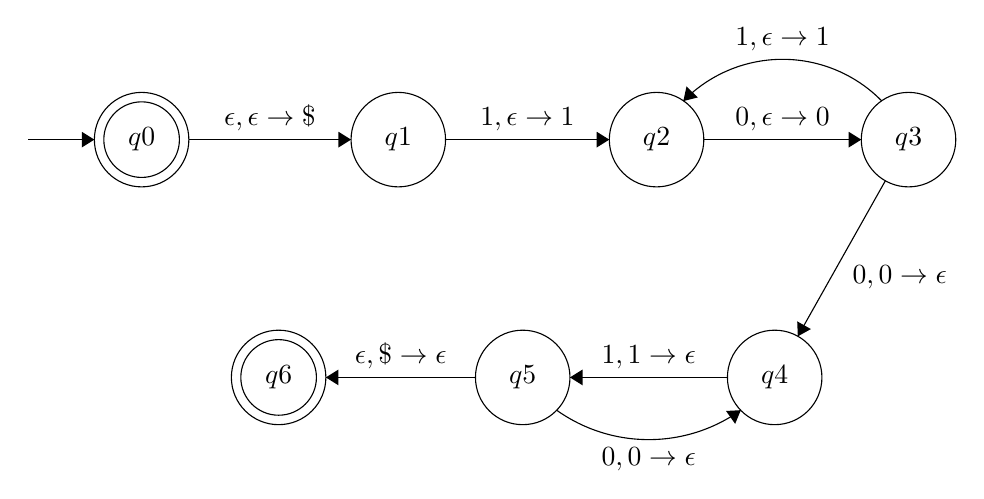
\begin{tikzpicture}[scale=0.2]
\tikzstyle{every node}+=[inner sep=0pt]
\draw [black] (18.8,-17.1) circle (3);
\draw (18.8,-17.1) node {$q0$};
\draw [black] (18.8,-17.1) circle (2.4);
\draw [black] (35.1,-17.1) circle (3);
\draw (35.1,-17.1) node {$q1$};
\draw [black] (51.5,-17.1) circle (3);
\draw (51.5,-17.1) node {$q2$};
\draw [black] (67.5,-17.1) circle (3);
\draw (67.5,-17.1) node {$q3$};
\draw [black] (59,-32.2) circle (3);
\draw (59,-32.2) node {$q4$};
\draw [black] (43,-32.2) circle (3);
\draw (43,-32.2) node {$q5$};
\draw [black] (27.5,-32.2) circle (3);
\draw (27.5,-32.2) node {$q6$};
\draw [black] (27.5,-32.2) circle (2.4);
\draw [black] (11.6,-17.1) -- (15.8,-17.1);
\fill [black] (15.8,-17.1) -- (15,-16.6) -- (15,-17.6);
\draw [black] (21.8,-17.1) -- (32.1,-17.1);
\fill [black] (32.1,-17.1) -- (31.3,-16.6) -- (31.3,-17.6);
\draw (26.95,-16.6) node [above] {$\epsilon,\epsilon \rightarrow \$$};
\draw [black] (38.1,-17.1) -- (48.5,-17.1);
\fill [black] (48.5,-17.1) -- (47.7,-16.6) -- (47.7,-17.6);
\draw (43.3,-16.6) node [above] {$1,\epsilon \rightarrow 1$};
\draw [black] (54.5,-17.1) -- (64.5,-17.1);
\fill [black] (64.5,-17.1) -- (63.7,-16.6) -- (63.7,-17.6);
\draw (59.5,-16.6) node [above] {$0,\epsilon \rightarrow 0$};
\draw [black] (53.2,-14.645) arc (135.56148:44.43852:8.824);
\fill [black] (53.2,-14.65) -- (54.12,-14.42) -- (53.4,-13.72);
\draw (59.5,-11.5) node [above] {$1,\epsilon \rightarrow 1$};
\draw [black] (56,-32.2) -- (46,-32.2);
\fill [black] (46,-32.2) -- (46.8,-32.7) -- (46.8,-31.7);
\draw (51,-31.7) node [above] {$1,1\rightarrow \epsilon$};
\draw [black] (56.851,-34.277) arc (-54.50521:-125.49479:10.077);
\fill [black] (56.85,-34.28) -- (55.91,-34.33) -- (56.49,-35.15);
\draw (51,-36.65) node [below] {$0,0\rightarrow \epsilon$};
\draw [black] (40,-32.2) -- (30.5,-32.2);
\fill [black] (30.5,-32.2) -- (31.3,-32.7) -- (31.3,-31.7);
\draw (35.25,-31.7) node [above] {$\epsilon, \$ \rightarrow \epsilon$};
\draw [black] (66.03,-19.71) -- (60.47,-29.59);
\fill [black] (60.47,-29.59) -- (61.3,-29.13) -- (60.43,-28.64);
\draw (63.91,-25.86) node [right] {$0,0\rightarrow \epsilon$};
\end{tikzpicture}
\end{center}

\pagebreak

\subsection{C}

Parsing Input: 10100101

$\newline$
\begin{tabular}{|l|l|l|l|l|l|l|l|l|l|l|l|l|l|l|}
\hline
Input: &    &   &  &  &  &  &  &  &  &  &  &  &  &  \\ \hline
Stack: & \$ & $\epsilon$ &  &  &  &  &  &  &  &  &  &  &  &  \\ \hline
\end{tabular}
$[(q_{0} \rightarrow q_{1}): \epsilon , \epsilon \rightarrow \$]$

$\newline$
\begin{tabular}{|l|l|l|l|l|l|l|l|l|l|l|l|l|l|l|}
\hline
Input: & \textbf{1} &   &  &  &  &  &  &  &  &  &  &  &  &  \\ \hline
Stack: & \textbf{1} & \$ & $\epsilon$ &  &  &  &  &  &  &  &  &  &  &  \\ \hline
\end{tabular}
$[(q_{1} \rightarrow q_{2}): 1 , \epsilon \rightarrow 1]$

$\newline$
\begin{tabular}{|l|l|l|l|l|l|l|l|l|l|l|l|l|l|l|}
\hline
Input: & 1 & \textbf{0}  &  &  &  &  &  &  &  &  &  &  &  &  \\ \hline
Stack: & \textbf{0} & 1 & \$ & $\epsilon$ &  &  &  &  &  &  &  &  &  &  \\ \hline
\end{tabular}
$[(q_{2} \rightarrow q_{3}): 0 , \epsilon \rightarrow 0]$

$\newline$
\begin{tabular}{|l|l|l|l|l|l|l|l|l|l|l|l|l|l|l|}
\hline
Input: & 1 & 0  & \textbf{1} &  &  &  &  &  &  &  &  &  &  &  \\ \hline
Stack: & \textbf{1} & 0 & 1 & \$ & $\epsilon$ &  &  &  &  &  &  &  &  &  \\ \hline
\end{tabular}
$[(q_{3} \rightarrow q_{2}): 1 , \epsilon \rightarrow 1]$

$\newline$
\begin{tabular}{|l|l|l|l|l|l|l|l|l|l|l|l|l|l|l|}
\hline
Input: & 1 & 0  & 1 & \textbf{0} &  &  &  &  &  &  &  &  &  &  \\ \hline
Stack: & \textbf{0} & 1 & 0 & 1 & \$ & $\epsilon$ &  &  &  &  &  &  &  &   \\ \hline
\end{tabular}
$[(q_{2} \rightarrow q_{3}): 0 , \epsilon \rightarrow 0]$

$\newline$
\begin{tabular}{|l|l|l|l|l|l|l|l|l|l|l|l|l|l|l|}
\hline
Input: & 1 & 0  & 1 & 0 & \textbf{0} &  &  &  &  &  &  &  &  &  \\ \hline
Stack: & 1 & 0 & 1 & \$ & $\epsilon$ &  &  &  &  &  &  &  & &   \\ \hline
\end{tabular}
$[(q_{3} \rightarrow q_{4}): 0 , 0 \rightarrow \epsilon]$

$\newline$
\begin{tabular}{|l|l|l|l|l|l|l|l|l|l|l|l|l|l|l|}
\hline
Input: & 1 & 0  & 1 & 0 & 0 & \textbf{1} &  &  &  &  &  &  &  &  \\ \hline
Stack: & 0 & 1 & \$ & $\epsilon$ &  &  &  &  &  &  &  & & &   \\ \hline
\end{tabular}
$[(q_{4} \rightarrow q_{5}): 1 , 1 \rightarrow \epsilon]$

$\newline$
\begin{tabular}{|l|l|l|l|l|l|l|l|l|l|l|l|l|l|l|}
\hline
Input: & 1 & 0  & 1 & 0 & 0 & 1 & \textbf{0} &  &  &  &  &  &  &  \\ \hline
Stack: & 1 & \$ & $\epsilon$ &  &  &  &  &  &  &  & & & &   \\ \hline
\end{tabular}
$[(q_{5} \rightarrow q_{4}): 0 , 0 \rightarrow \epsilon]$

$\newline$
\begin{tabular}{|l|l|l|l|l|l|l|l|l|l|l|l|l|l|l|}
\hline
Input: & 1 & 0  & 1 & 0 & 0 & 1 & 0 & \textbf{1} &  &  &  &  &  &  \\ \hline
Stack: & \$ & $\epsilon$ &  &  &  &  &  &  &  & & & & &   \\ \hline
\end{tabular}
$[(q_{4} \rightarrow q_{5}): 1 , 1 \rightarrow \epsilon]$

$\newline$
\begin{tabular}{|l|l|l|l|l|l|l|l|l|l|l|l|l|l|l|}
\hline
Input: & 1 & 0  & 1 & 0 & 0 & 1 & 0 & 1 &  &  &  &  &  &  \\ \hline
Stack: & $\epsilon$ &  &  &  &  &  &  &  & & & & & &   \\ \hline
\end{tabular}
$[(q_{5} \rightarrow q_{6}): \epsilon , \$ \rightarrow \epsilon]$

$\newline$
Input Accepted.

\pagebreak

\section{}

\subsection{A}

Grammar for $L_{1} = \{1^n0^{2n}|n\geq0\}$ :

$S \rightarrow 1S00 | \epsilon$

\subsection{B}

Considering the string $w = 1^p0^{2p} \in L_{1}$:

For a split into the parts $uvxyz$, the pump-able segment $v$ must consist of only $1$, so $v = 1$ and segment $y$ must consist of only $00$, $y=00$. So when you pump both segments as follows: $uv^ixy^iz$ $\forall i \geq 0$ the condition that there are two times as many 0's as 1's will hold.

\subsection{C}

Considering the string $w = 1^p0^{2p}1^p \in L_{1}$:

There are a number of possible cases for a split into the parts $uvxyz$.

One is that the pump-able segment $v$ would consist of $1$, so $v = 1$ and segment $y$ would consist of $00$, so $y=00$. This is not pump-able since the succeeding number of 1's wont equal the preceding number.

Another is that the pump-able segment $v$ would consist of $10$, so $v = 10$ and segment $y$ would consist of $1$, so $y=1$. This is not pump-able since the succeeding number of 0's wont be twice the number of preceding and succeeding 1's.

Another is that the pump-able segment $v$ would consist of $1$, so $v = 1$ and segment $y$ would consist of $01$, so $y=01$. This is not pump-able since the number of 0's wont be twice the number of preceding and succeeding 1's and they would be out of order.

Another is that the pump-able segment $v$ would consist of $10$, so $v = 10$ and segment $y$ would consist of $01$, so $y=01$. This is not pump-able since the values would be out of order.

So in any condition, if you pump both segments as follows: $uv^ixy^iz$ $\forall i \geq 0$ the condition that there are $n$ 1's followed by $2n$ 0's followed by $n$ 1's again can't possibly hold.

\end{document}
%%%%%%%%%%%%%%%%%%%%%%%%%%%%%%%%%%%%%%%%%%%%%%%%%%%%%%%%%%%%%%%%%%%%%%

